\section{Atombau}

\subsection{Atome}
Atome bestehen aus Atomkern ($p^+$, $n$) und Atomhülle ($e^-$).

\begin{table}[htbp]
	\begin{tabular}{|l|c|c|}
		Elementarteilchen & Masse & El. Ladung \\ \hline
		Proton $p^+$ & 1.0073 u & 1+ \\
		Neutron $n$ & 1.0087 u & 0 \\
		Elektron $e^-$ & 0.0005 u & 1- \\ \hline
	\end{tabular}
\end{table}

Atomare Masseinheit $u$: $\frac{1}{12}$ der Masse eines C-12 Atoms. \\

Elementarladung $e$: $\pm 1.602 \cdot 10^{-19} C$ ($C$: Coulomb) \\

Schreibweise von Atomen: $ ^\text{Atommasse}_\text{Ordnungszahl} X ^\text{Ladung}$ \\

\subsection{Isotope}
Atome eines Elements, die sich in ihrer Neutronenzahl unterscheiden.

\subsection{Elektronen}
Elektronen befinden sich auf bestimmten, diskreten Energieniveaus (Schalen: K,L,M,N,...). 

\begin{figure}[htbp]
	\centering
	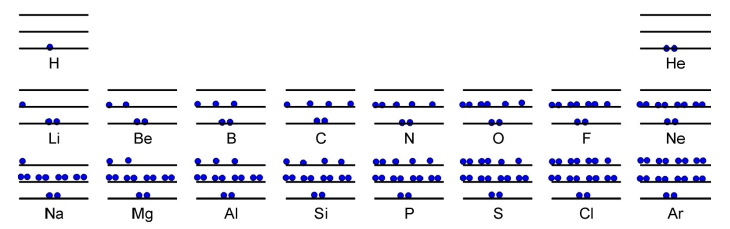
\includegraphics[width=0.9\linewidth]{images/2_Energie_der_Elektronen.png}
\end{figure}

Ionisierungsenergie $E_{Ion}$: Energie, welche benötigt wird um ein $e^-$ vollständig aus einem Atom zu entfernen.\\

Maximale Anzahl $e^-$ pro Energieniveau: $2 \cdot n^2$ (n: Nummer des Energieniveaus) \\

Valenzelektronen: Elektronen des höchsten Energieniveaus. Zahl der VE bestimmt chem. Eigenschaften eines Elements \\
Atomrumpf: Atom ohne Valenzelektronen \\
Rumpfladung: Ladung des Atomrumpfs \\

Energieniveaus werden aufgrund der Abstossung der $e^-$ in Unterniveaus (s,p,d,f,...) aufgeteilt. Unterniveaus verschiedener Hauptniveaus können sich überlappen (z.B. 4s liegt tiefer als 3d).

\subsection{Orbitalmodell}
Welle-Teilchen-Dualismus $\Rightarrow$ $e^-$ können als stehende Welle betrachtet werden. \\

Orbital: Raum, in dem sich ein $e^-$ mit grösster Wahrscheinlichkeit aufhält. \\

\subsubsection{Regeln für Elektronenkonfiguration}
\begin{enumerate}
	\item Besetzung der Orbitale mit $e^-$ nach aufsteigender Energie.
	\item Pauli-Prinzip: max. 2 $e^-$ pro Orbital.
	\item Hund'sche Regel: Orbitale mit gleicher Ordnung werden zuerst mit 1 $e^-$ besetzt.
\end{enumerate}

\begin{figure}[htbp]
	\centering
	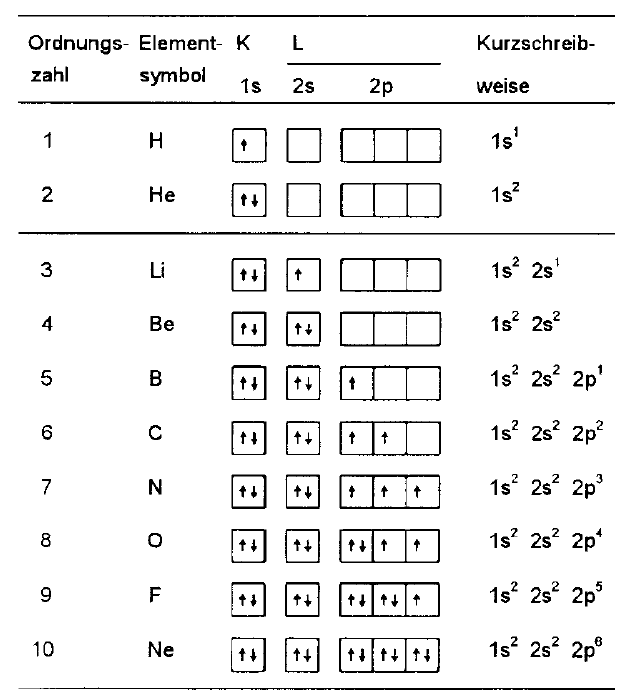
\includegraphics[width=0.75\linewidth]{images/2_Konfiguration_Orbitale.png}
\end{figure}

\subsection{Lewis-Schreibweise}
Meist spielen nur Valenzelektronen eine Rolle $\Rightarrow$ nur VE zeichnen.
\begin{figure}[htbp]
	\centering
	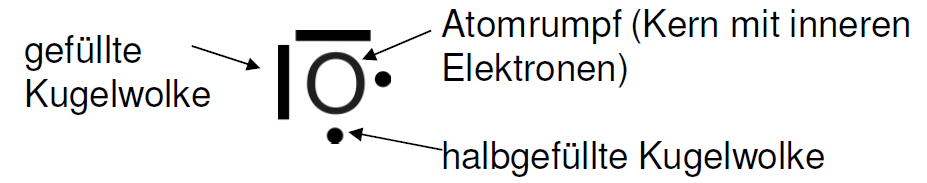
\includegraphics[width=0.5\linewidth]{images/2_Lewis_Schreibweise.png}
\end{figure}

\subsection{Edelgasregel}
Alle Atome sind bestrebt eine Edelgaskonfiguration zu erreichen, d.h. 8 VE. Ausnahmen: H, He.

\begin{itemize}
	\item Metallatome: Abgabe von $e^-$ (kl. Rumpfladung) $\Rightarrow$ Kationen
	\item Nichtmetallatome: Aufnahme von $e^-$ $\Rightarrow$ Anionen, oder Teilen von $e^-$ mit anderen Atomen (Moleküle)
\end{itemize}